\section{Random\-Tree  Class Reference}
\label{classRandomTree}\index{RandomTree@{Random\-Tree}}
Naively extend the tree by random node selection (not really an {\bf RRT} {\rm (p.\,\pageref{classRRT})}). 


{\tt \#include $<$rrt.h$>$}

Inheritance diagram for Random\-Tree::\begin{figure}[H]
\begin{center}
\leavevmode
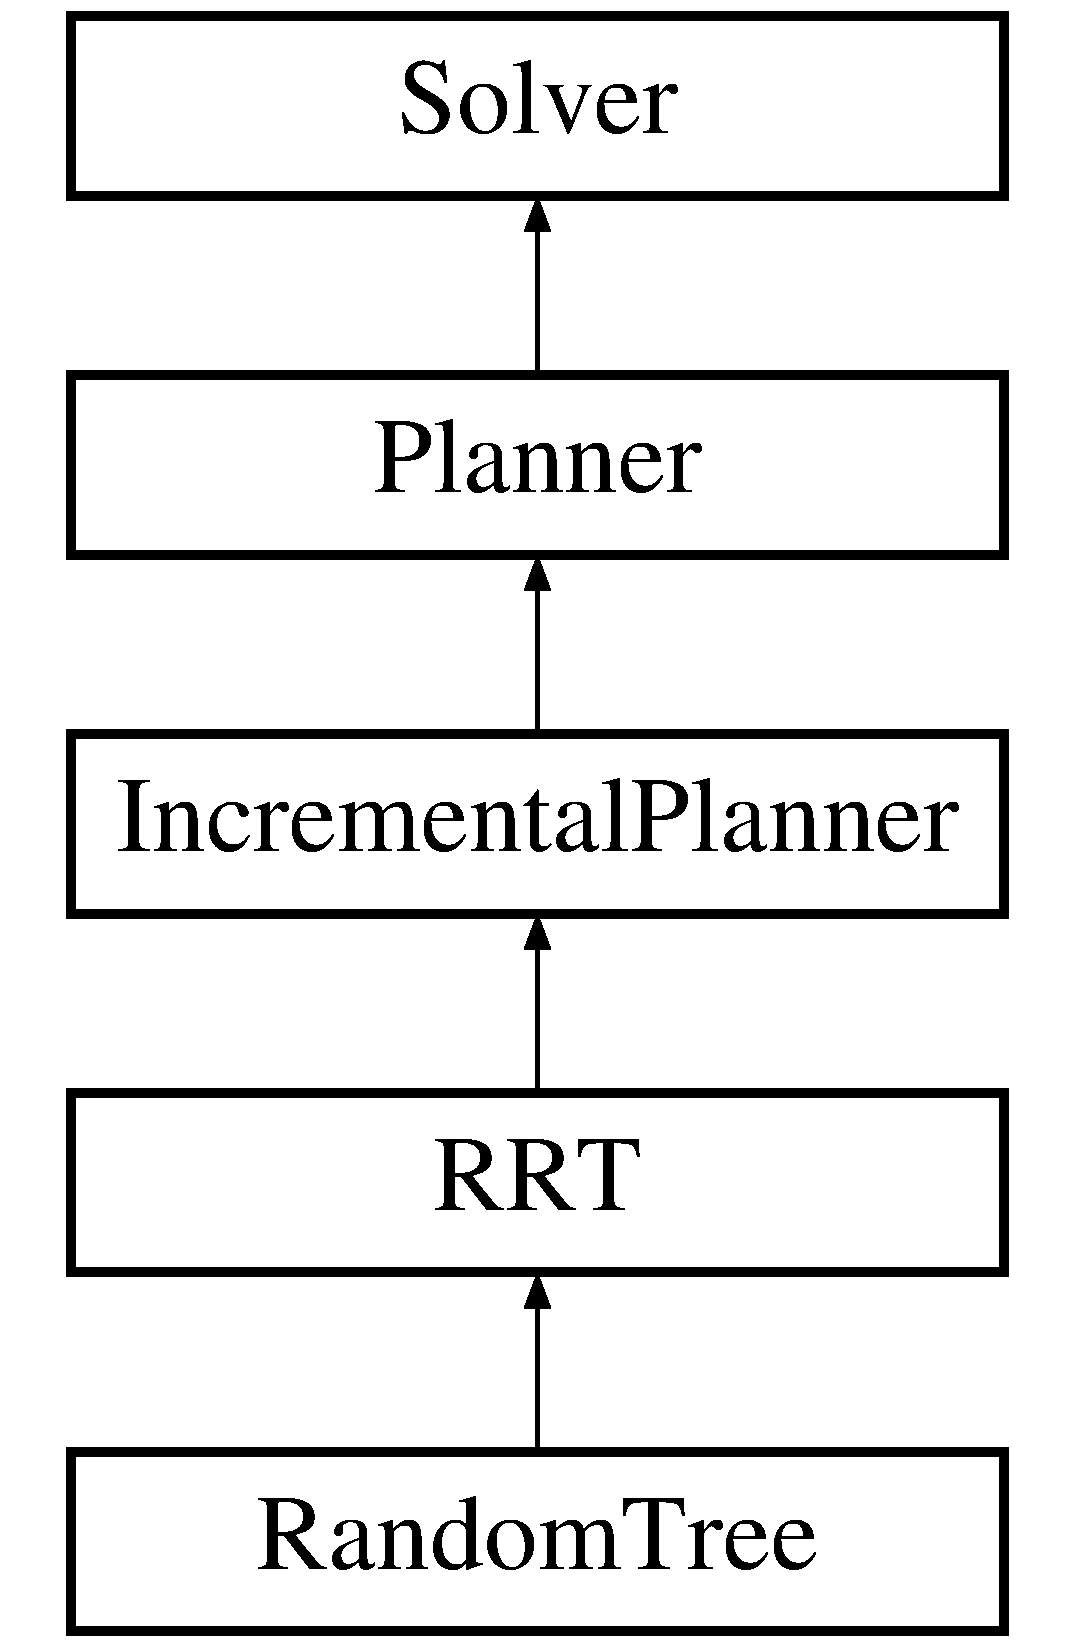
\includegraphics[height=5cm]{classRandomTree}
\end{center}
\end{figure}
\subsection*{Public Methods}
\begin{CompactItemize}
\item 
{\bf Random\-Tree} ({\bf Problem} $\ast$p)
\item 
virtual {\bf $\sim$Random\-Tree} ()
\end{CompactItemize}
\subsection*{Protected Methods}
\begin{CompactItemize}
\item 
virtual {\bf MSLNode} $\ast$ {\bf Select\-Node} (const {\bf MSLVector} \&{\bf x}, {\bf MSLTree} $\ast$t, bool forward)
\begin{CompactList}\small\item\em Return the nearest neighbor in the graph.\item\end{CompactList}\item 
virtual {\bf MSLVector} {\bf Select\-Input} (const {\bf MSLVector} \&x1, const {\bf MSLVector} \&x2, {\bf MSLVector} \&nx\_\-best, bool \&success, bool forward)
\begin{CompactList}\small\item\em Select the input that gets closest to x2 from x1.\item\end{CompactList}\end{CompactItemize}


\subsection{Detailed Description}
Naively extend the tree by random node selection (not really an {\bf RRT} {\rm (p.\,\pageref{classRRT})}).

Grow a tree incrementally by simply selecting vertex at random and  moving in a random direction from the chosen vertex. It is not  really a Rapidly-exploring Random Tree since there is no random sampling over the state space to \char`\"{}pull\char`\"{} the tree. 



\subsection{Constructor \& Destructor Documentation}
\index{RandomTree@{Random\-Tree}!RandomTree@{RandomTree}}
\index{RandomTree@{RandomTree}!RandomTree@{Random\-Tree}}
\subsubsection{\setlength{\rightskip}{0pt plus 5cm}Random\-Tree::Random\-Tree ({\bf Problem} $\ast$ {\em p})}\label{classRandomTree_a0}


\index{RandomTree@{Random\-Tree}!~RandomTree@{$\sim$RandomTree}}
\index{~RandomTree@{$\sim$RandomTree}!RandomTree@{Random\-Tree}}
\subsubsection{\setlength{\rightskip}{0pt plus 5cm}virtual Random\-Tree::$\sim$Random\-Tree ()\hspace{0.3cm}{\tt  [inline, virtual]}}\label{classRandomTree_a1}




\subsection{Member Function Documentation}
\index{RandomTree@{Random\-Tree}!SelectInput@{SelectInput}}
\index{SelectInput@{SelectInput}!RandomTree@{Random\-Tree}}
\subsubsection{\setlength{\rightskip}{0pt plus 5cm}{\bf MSLVector} Random\-Tree::Select\-Input (const {\bf MSLVector} \& {\em x1}, const {\bf MSLVector} \& {\em x2}, {\bf MSLVector} \& {\em nx\_\-best}, bool \& {\em success}, bool {\em forward})\hspace{0.3cm}{\tt  [protected, virtual]}}\label{classRandomTree_b1}


Select the input that gets closest to x2 from x1.



Reimplemented from {\bf RRT} {\rm (p.\,\pageref{classRRT_b0})}.\index{RandomTree@{Random\-Tree}!SelectNode@{SelectNode}}
\index{SelectNode@{SelectNode}!RandomTree@{Random\-Tree}}
\subsubsection{\setlength{\rightskip}{0pt plus 5cm}{\bf MSLNode} $\ast$ Random\-Tree::Select\-Node (const {\bf MSLVector} \& {\em x}, {\bf MSLTree} $\ast$ {\em t}, bool {\em forward})\hspace{0.3cm}{\tt  [protected, virtual]}}\label{classRandomTree_b0}


Return the nearest neighbor in the graph.



Reimplemented from {\bf RRT} {\rm (p.\,\pageref{classRRT_b1})}.

The documentation for this class was generated from the following files:\begin{CompactItemize}
\item 
{\bf rrt.h}\item 
{\bf rrt.C}\end{CompactItemize}
